% $Id: board1.tex 9376 2021-08-31 13:12:43Z mskala $

%
% MSK 008 Board 1 build instructions
% Copyright (C) 2017, 2018  Matthew Skala
%
% This program is free software: you can redistribute it and/or modify
% it under the terms of the GNU General Public License as published by
% the Free Software Foundation, version 3.
%
% This program is distributed in the hope that it will be useful,
% but WITHOUT ANY WARRANTY; without even the implied warranty of
% MERCHANTABILITY or FITNESS FOR A PARTICULAR PURPOSE.  See the
% GNU General Public License for more details.
%
% You should have received a copy of the GNU General Public License
% along with this program.  If not, see <http://www.gnu.org/licenses/>.
%
% Matthew Skala
% https://northcoastsynthesis.com/
% mskala@northcoastsynthesis.com
%

\chapter{Building Board 1}\label{ch:board1}

Board~1 has components on both sides, and for best results, it is important
to install them in the right order.  Build Board~2 first, and see the
general comments in the Board~2 chapters about how to approach the task.

\section{Preliminaries}

Count out the right number of everything according to the bill of materials. 
There is an abbreviated BOM for the items needed in this chapter (including
the final assembly of the module) in Table~\ref{tab:b1bom}.  It
is also assumed you have a finished Board~2 from the previous chapter.

\noindent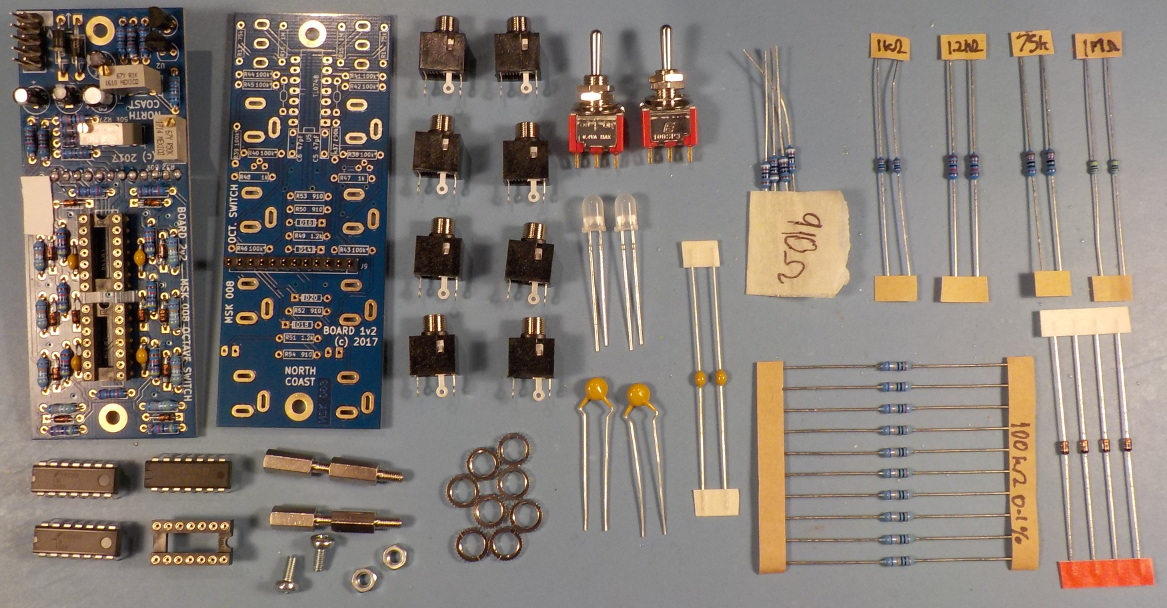
\includegraphics[width=\linewidth]{board1-parts.jpg}

\begin{table*}
{\centering
\fbox{This table is not a substitute for the text instructions.}
\vspace{\baselineskip}

\begin{tabular}{rp{1.3in}cp{3in}}
  \textbf{Qty} & \textbf{Ref} & \textbf{Value/Part No.} & \\ \hline
\input{bomdata-1.tex}
\end{tabular}\par}
\caption{Bill of Materials for Board~1.}\label{tab:b1bom}
\end{table*}

If you wish to reconfigure the CV2 inputs, you can change the solder jumpers
on Board~1 at this point.  In a standard build, the CV2 input on the left
channel \emph{adds} its voltage to CV1 and the quantizer output, while the
CV2 input on the right channel \emph{subtracts}.  This configuration is the
most useful one for most users and it is not particularly recommended to
change it.  But if you want to, first locate the jumpers on the board.  JP1
on the left is for the left channel and JP2 on the right is for the right
channel.

\noindent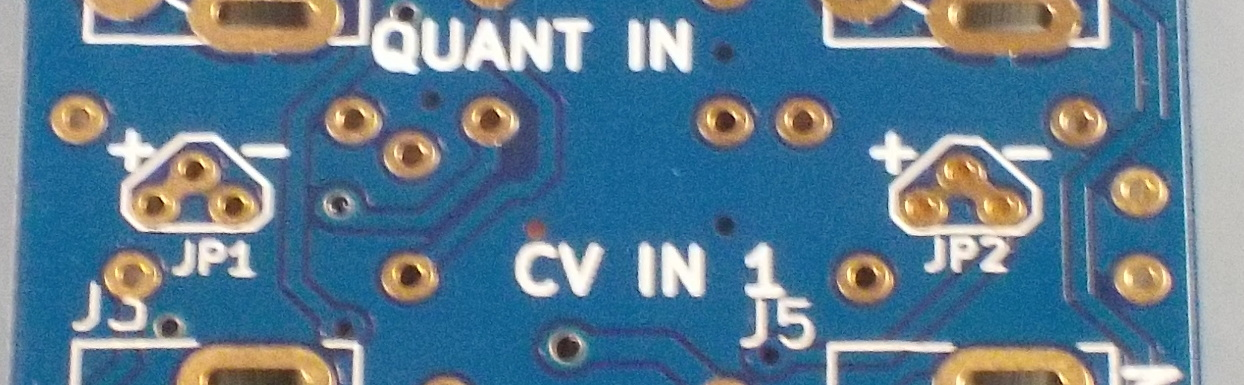
\includegraphics[width=\linewidth]{jumpers.jpg}

Each jumper has three terminals.  The middle one is connected to the one on
the left or the right for positive (adding) or negative (subtracting)
respectively, with a default set by a trace built into the circuit board. 
To change the jumper, use a sharp knife to carefully cut the connecting
trace, and then apply a blob of solder connecting the middle terminal to the
one for the opposite selection.  Use an ohmmeter to check that you have
really broken the connection on one side and recreated it on the other.

For a more advanced modification, you can solder fine wires into the holes
provided and run them into other circuitry of your own construction.  If you
add an SPDT switch, you could use it to change the add/subtract option by
flipping the switch.  You could also connect any number of additional
inverting and noninverting input jacks through 100k$\Omega$ precision
resistors (0.1\%\ or better) to the $+$ and $-$ terminals, which as shown on
the schematic diagram are op amp virtual ground summing nodes.

\section{Decoupling capacitors}

The two axial ceramic 0.1$\mu$F decoupling capacitors C7 and C8 are shown on
the board by a special symbol without their reference designators.

\noindent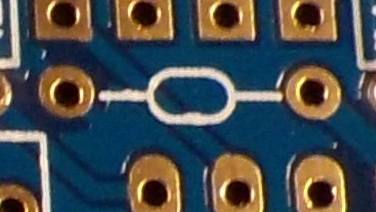
\includegraphics[width=\linewidth]{decoup-symbol.jpg}

\pagebreak

Install these two capacitors where the symbol appears.  They are not
polarized and may be installed in either orientation.  These capacitors act
as filters for the power supplies to the op amp chip, protecting them from
high-frequency crosstalk.

\noindent\includegraphics[width=\linewidth]{{cap-0.1u1}.jpg}

\section{Fixed resistors}

Resistors are never polarized.  I like to install mine in a consistent
direction for cosmetic reasons, but this is electrically unnecessary.  In
this module, most resistors are metal film 1\%\ type; a few are 0.1\%\
precision metal film resistors.  Both kinds will usually have blue bodies
and four colour bands designating the value, plus a fifth band for the
tolerance, and these are the resistors shipped in the North Coast
kits.  The tolerance band is brown for 1\%\ and violet for 0.1\%, but note
that we may occasionally ship better-tolerance resistors in the kits than
the specifications require, if we are able to source them at a good price.
Accordingly, I mention only the four value band colours for this type of
resistor; if you are using resistors with other codes, you are responsible
for knowing them.  Note that colour codes on metal film 1\% resistors are
often ambiguous (reading from one end or the other end may give two
different values, both plausible) and some of the colours are hard to
distinguish anyway.  If in doubt, always measure with an ohmmeter before
soldering the resistor in place.

There are no cases in this module of the same nominal resistance value being
used at more than one tolerance, but the 0.1\%\ resistance values are marked
with asterisks (*) on the board silkscreen as a reminder that these
positions require special resistors.

The physical size of the resistors may vary, and details like the exact
colour of the bluish background.  You can see some of that variation in the
photos in these instructions.  Some of the resistance values used in this
module are hard to find, and we source different values from different
suppliers, so not all the resistors in a kit will necessarily be from the
same manufacturer, nor match on non-critical specifications like power
rating and physical size.

Install the four 910$\Omega$ (white-brown-black-black) resistors R50, R52,
R53, and R54.  These form part of the current-controlling network for the
LED drivers.

\noindent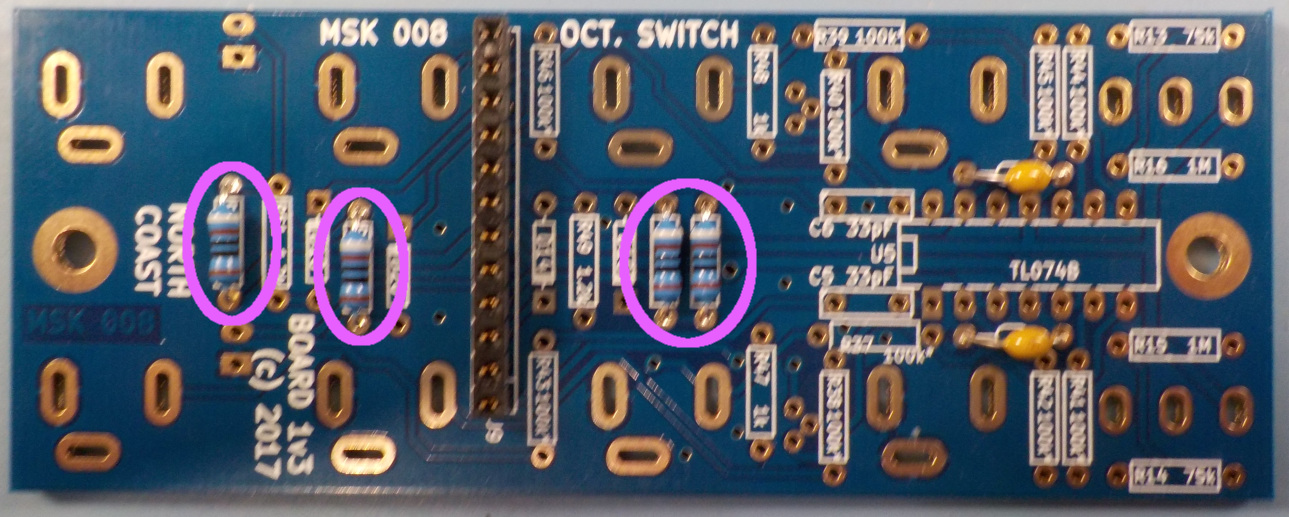
\includegraphics[width=\linewidth]{res-910.jpg}

Install the two 1k$\Omega$ (brown-black-black-brown) resistors R47 and R48. 
These are current-limiting resistors to protect external circuits from
excessive output power on the module outputs; they also serve to isolate the
op amp chip from reactive (capacitive or inductive) loads that could make it
unstable.  Do not confuse these resistors with other power-of-ten values
such as 100k$\Omega$, which also have codes starting brown-black-black but
with different colours for the fourth, exponent-indicating, colour band.

\noindent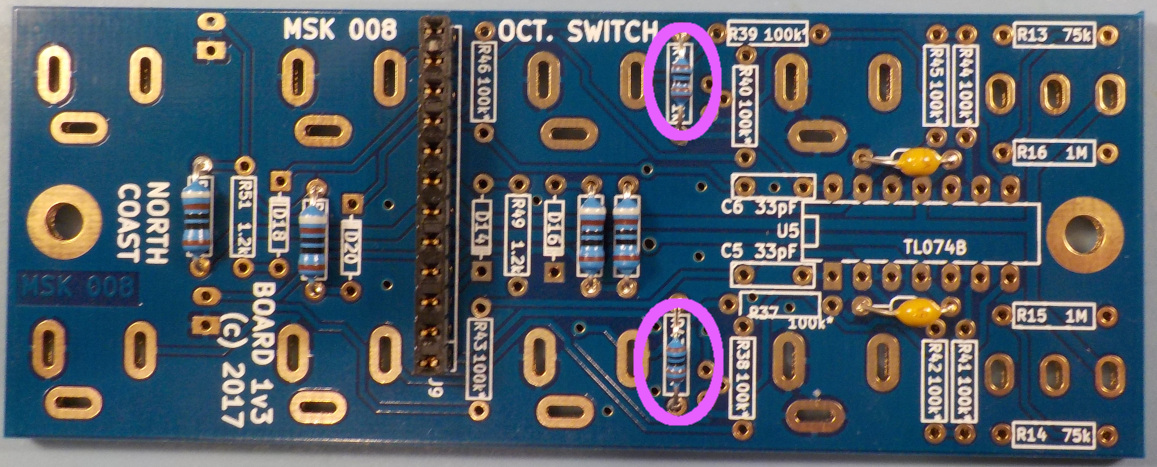
\includegraphics[width=\linewidth]{res-1k.jpg}

Install the two 1.2k$\Omega$ (brown-red-black-brown) resistors R49 and R51. 
These form part of the current-controlling network for the LED drivers.

\noindent\includegraphics[width=\linewidth]{{res-1.2k}.jpg}

\pagebreak

Install the two 75k$\Omega$ (violet-green-black-red) resistors R13 and R16. 
These set the weight of the quantizer voltage inputs in comparison to the
manual octave switches.

\noindent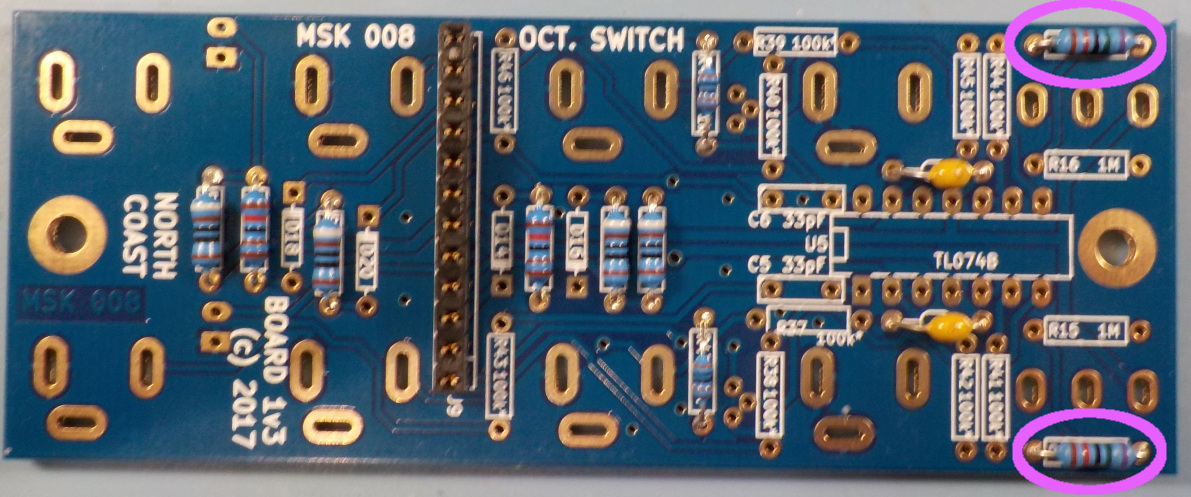
\includegraphics[width=\linewidth]{res-75k.jpg}

Install the two 1M$\Omega$ (brown-black-black-yellow) resistors R15 and R16. 
These set the weight of the manual octave switches in the quantizers.  Do
not confuse them with other power-of-ten resistance values.

\noindent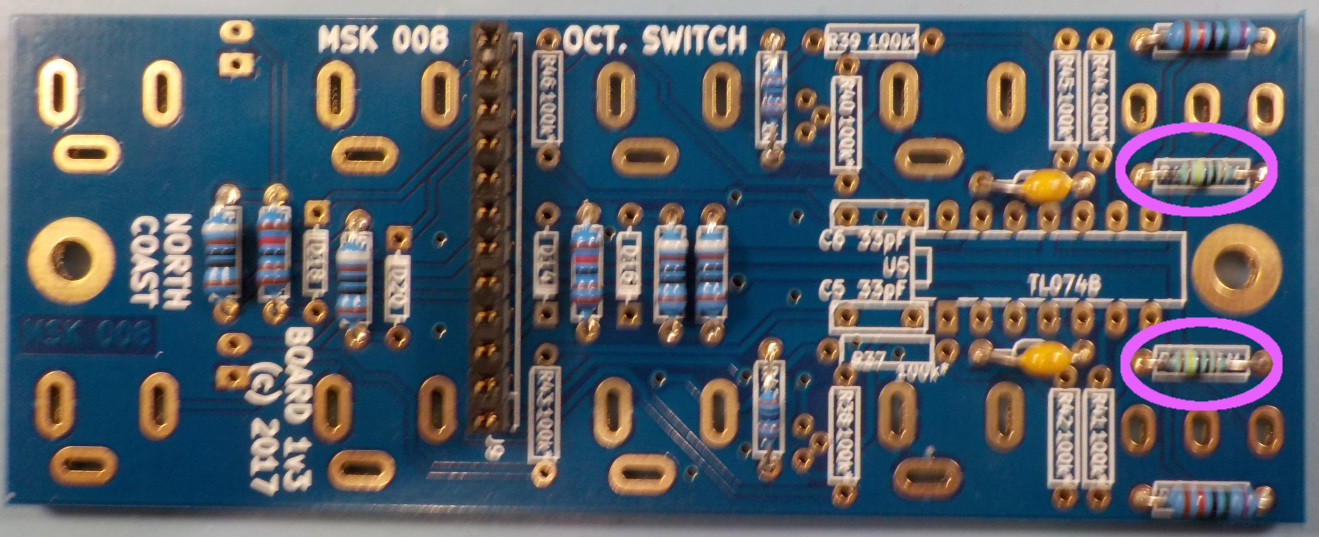
\includegraphics[width=\linewidth]{res-1M.jpg}

Install the ten 100k$\Omega$ 0.1\%\ precision resistors.  These control the
gain of the summing and inversion op amp circuits.  When building the
prototypes I noticed that either these resistors are just a little larger
than others of the same approximate body size, or maybe their leads are a
little stiffer; I found that I needed to bend the leads tighter (closer to
the bodies) than usual in order to have them fit nicely on the board.  Take
it slowly and carefully.

\noindent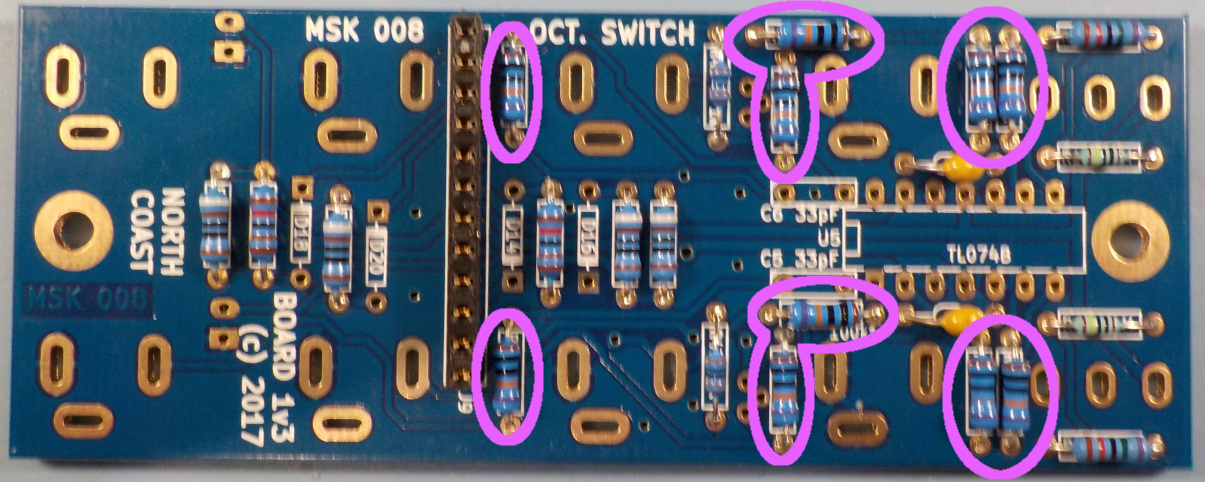
\includegraphics[width=\linewidth]{res-100k.jpg}

\section{Semiconductors}

Install the four 1N4148 or 1N914 switching diodes D14, D16, D18, and D20,
and D19.  These switch the LED drive currents.
They are polarized components and it is important to
install them right way round.  Each diode is packaged inside a pink glass
bead with a black stripe at one end; that end is the \emph{cathode}.  The
silkscreen markings on the board have a corresponding stripe and the diodes
should be installed with their stripes matching the markings on the board. 
The solder pads for the cathodes are also square instead of round. 
Installing one or more of these diodes backwards will result in incorrect
operation of the LEDs.

\noindent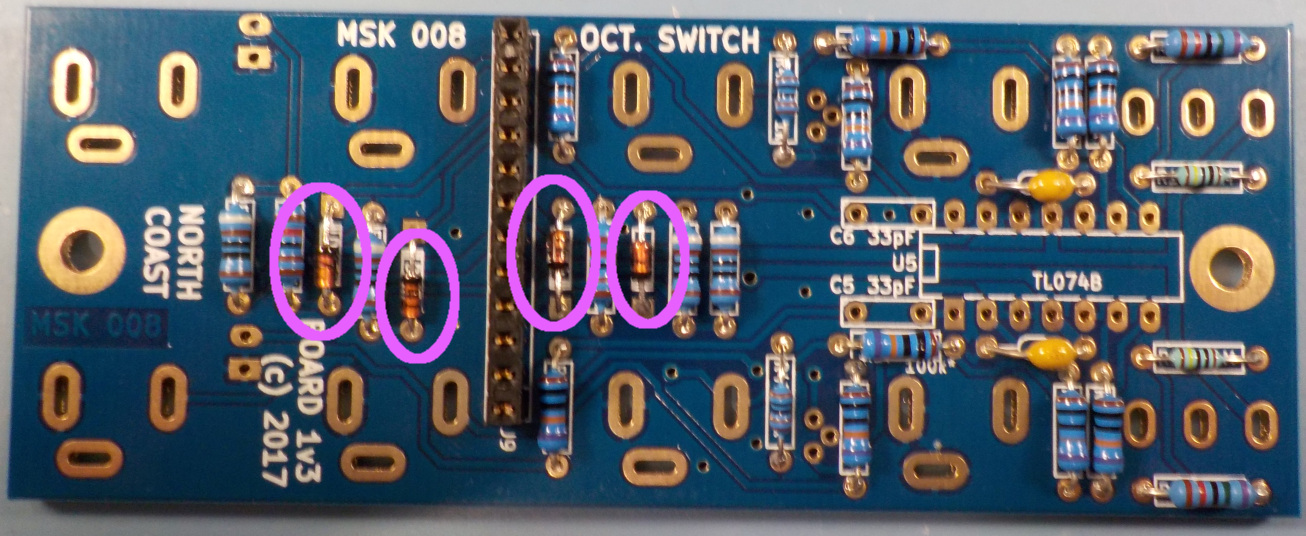
\includegraphics[width=\linewidth]{diodes1.jpg}

Install the 14-pin DIP socket for the TL074B quad low-offset operational
amplifier (op amp) U5.  This chip processes the CV1 and CV2 inputs,
inverting them as necessary, and does the final summation to drive the
module output.  The socket itself does not care which direction you install
it, but it is critically important that the chip installed in the socket
should be installed in the right direction.  To help with that, the socket
will probably be marked with a notch at one end (indicating the end where
Pin~1 and Pin~14 are located) and you should install the socket so that the
notched end matches the notch shown on the PCB silkscreen.  The solder pad
for Pin~1 is also distinguished by being rectangular instead of rounded.

Two of the holes for the capacitors C5 and C6 are located just off one end
of the DIP socket's footprint at the same spacing, making it possible to
insert the DIP socket shifted over one space with two of its pins in the
capacitor holes.  Be careful not to do that.

Installing DIP sockets without having them tilted at a funny angle can be
tricky.  I recommend inserting the socket in the board, taping it in place
on the component side with vinyl electrical tape, then soldering one pin on
one corner and checking that the socket is snug against the board before
soldering the other pins.  That way, if you accidentally solder the first
pin with the socket tilted, it will be easier to correct (only one pin to
desolder instead of all of them).

\noindent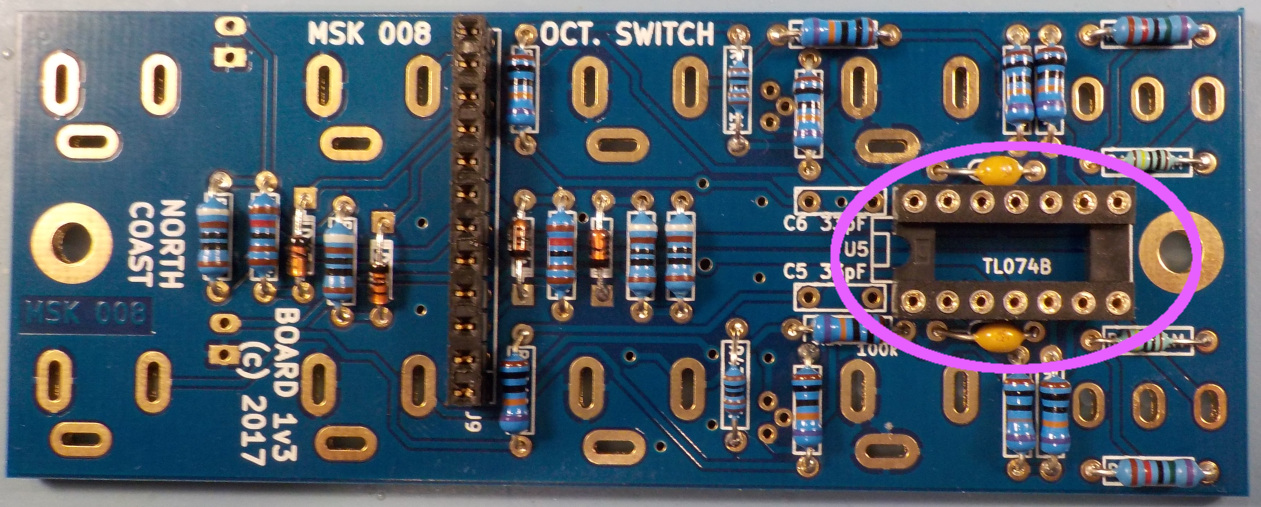
\includegraphics[width=\linewidth]{dip1.jpg}

\section{Compensation capacitors}

Install the two 33pF radial ceramic capacitors C5 and C6.  They will
probably be marked ``330,'' which means 33pF in a scheme similar to the
resistor colour code:  significant digits 3 3 to be followed by 0 zeroes. 
These capacitors help ensure stability of the op amp drivers by killing the
frequency response at ultrasonic frequencies, making parasitic oscillation
harder to sustain.

\noindent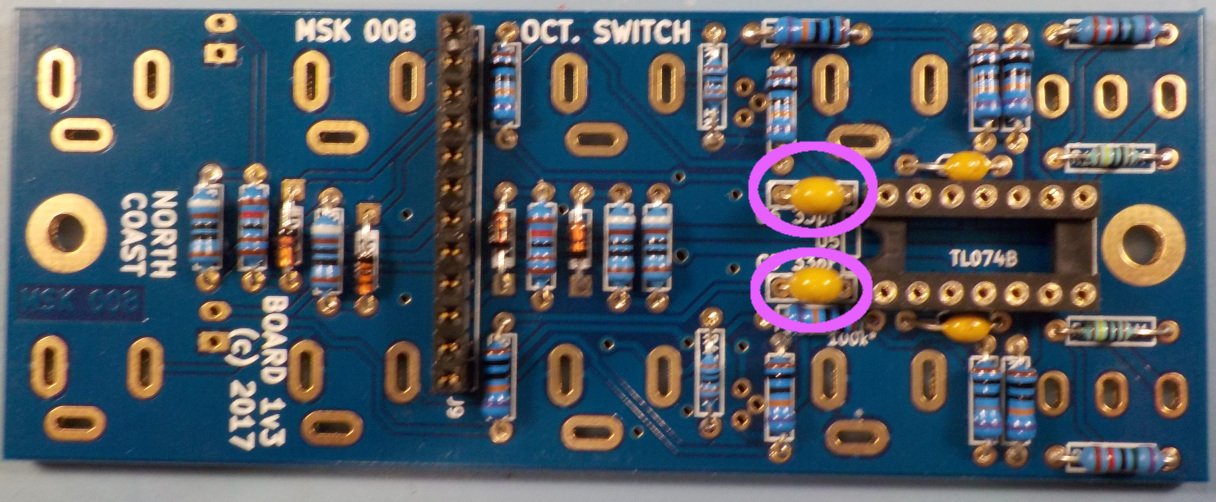
\includegraphics[width=\linewidth]{cap-33p.jpg}

\section{Panel components}

Fasten the 10mm and 11mm standoffs to Board~1.  The 11mm standoffs
should be on the same side of the board as the resistors and other
components, with their male ends sticking up as shown; they will separate
the two boards when the module is fully assembled.  The 10mm standoffs
should be on the other side, where they will separate the circuit boards
from the panel, with their male ends through the holes in the board to mate
with the 11mm standoffs.  \emph{Do not confuse the two similar lengths of
standoffs.}  Arranging them wrong at this stage may result in soldering panel
components at the wrong spacing in a way that will eventually make it
impossible to assemble the module correctly.
There is an exploded diagram for the final module on
page~\pageref{fig:exploded}.  You may wish to consult it if the way the
hardware fits together is at all unclear.

\noindent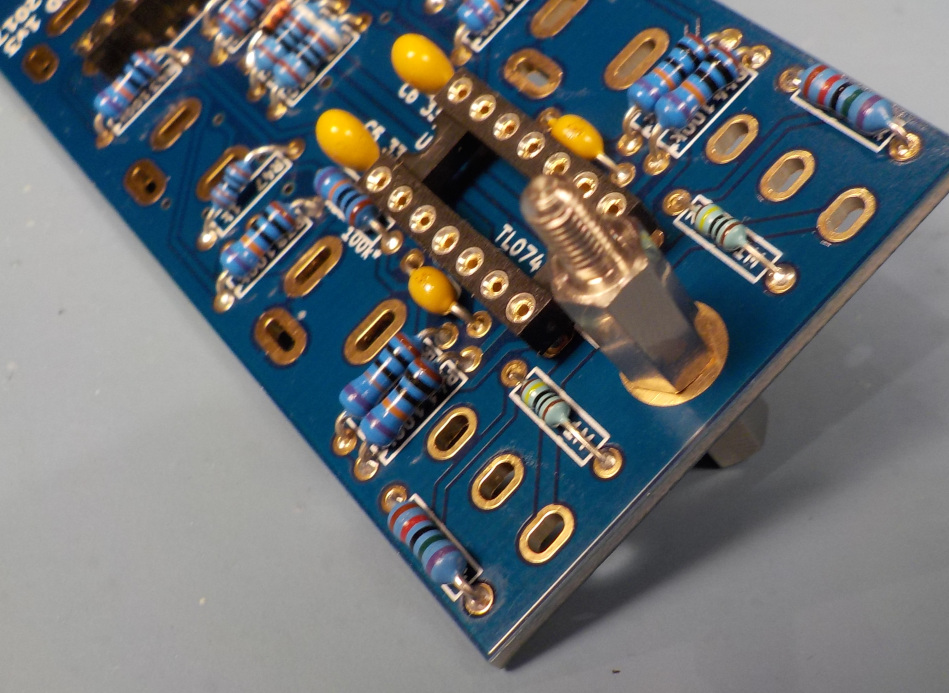
\includegraphics[width=\linewidth]{standoffs.jpg}

\pagebreak

Place (do not solder yet) the LEDs D11 and D12 in their corresponding holes
on the board.  Single LEDs are polarized and can be destroyed by reverse
voltage.  These ones here are special bi-colour devices with two separate
LEDs in each package.  The internal connection is such that each one
protects the other from reverse voltage; so if connected backwards, they
will not be destroyed, but the intended green and red colours will be
swapped.  Each LED lens has one flat side, and one leg shorter than the
other on that side.  The short leg is Pin~1.  Its proper place on the board
is marked by a circle with a flattened side matching the direction of the
flattened side on the LED lens, and an oval solder pad.  The other leg
(Pin~2, long, farther from the flat side) goes into the rectangular solder
pad.  Be sure both LEDs are placed right way around according to these
clues.

\noindent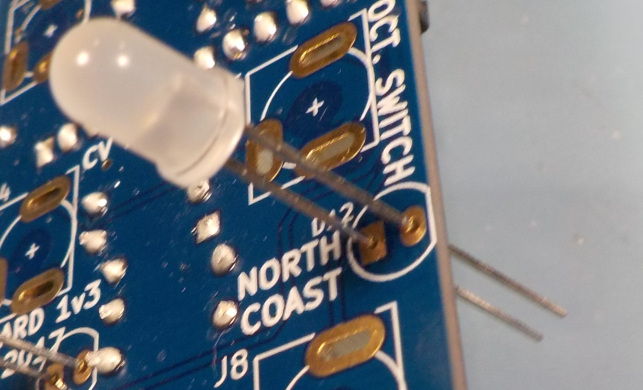
\includegraphics[width=\linewidth]{led.jpg}

Place (do not solder yet) the eight jack sockets J1 to J8 in their
corresponding holes on the board.  Their arrangement of legs and
corresponding slotted holes is such that they will only fit one way.

\noindent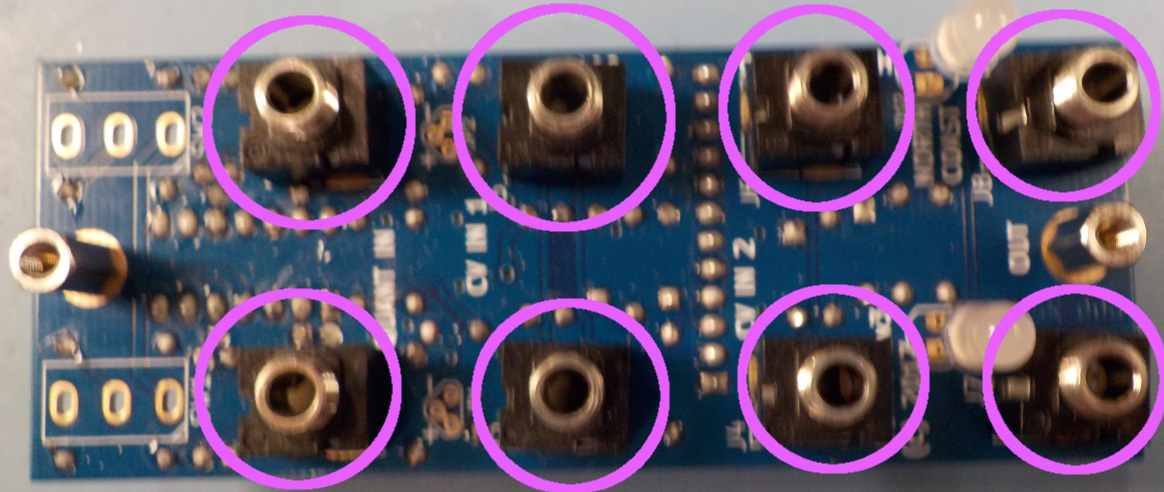
\includegraphics[width=\linewidth]{sockets.jpg}

Place (do not solder yet) the two toggle switches SW1 and SW2 in their
corresponding holes on the board.  The electrical connections on these
switches are symmetrical, but there is a keyway or groove on the threaded
bushing of each switch, and the keyway must be oriented downward for the
mounting hardware to fit properly later.

\noindent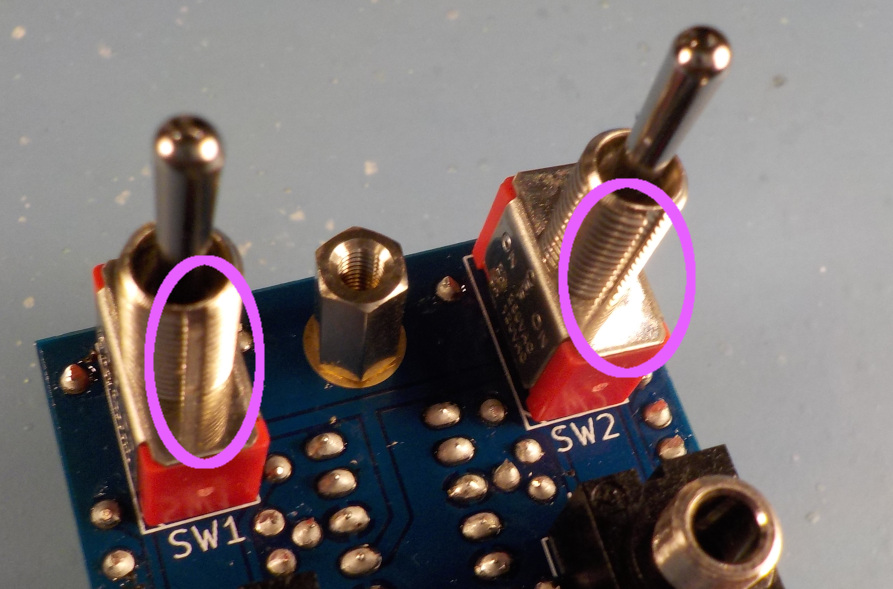
\includegraphics[width=\linewidth]{keyways.jpg}

Put the panel in place over the board so that the jack socket and toggle
switch bushings go through the corresponding holes in the panel and the
standoff line up behind their corresponding holes.  It may require some
careful adjustment of the jack socket locations to get them all through the
panel properly.  Check that the keyways on the toggle switch bushings are
facing downward, towards the small panel holes that will accept the tabs
from the locking rings.  Attach the panel firmly with the machine screws.

Use the knurled nuts that came with the jacks, to attach those to the panel. 
Beware of damaging the panel with wrenches, pliers, and similar.  If you
must use pliers, wrap them with tape to reduce the risk of scratches; but
just screwing the nuts on with finger pressure should be sufficient.

Use the hardware that came with the switches to attach them to the panel. 
In order starting closest to the panel, there should be a locking ring with
a tab that fits into the keyway on the switch bushing and another tab that
fits into the small hole on the panel; a toothed lockwasher; and at least
one hex nut.\footnote{These switches usually come with two nuts, but one is
probably sufficient given the use of the toothed lockwasher.} If the locking
ring will not fit because you mounted the switch backwards with the keyway
on the opposite side, this is your last chance to fix it.

Turn the assembly over so that the LEDs fall into place.  Adjust them by
gently pulling or pushing their legs until they all pass through the panel
holes by whatever amount you prefer.  If they are very loose, it may be
necessary to use sticky tape to temporarily hold them at the right depth,
but such a measure is unlikely to be needed; the holes are designed to be a
moderately snug friction fit on the LED lenses.

Solder all the jack sockets, LEDs, and switches.  The jack sockets and
switches may require a relatively large amount of solder to fill the
corresponding holes, but these joints are structural and should not be
neglected.  The LEDs, on the other hand, are sensitive to soldering heat and
should not be given excessive amounts of solder and heating, though the
joints must at least be strong enough not to break if users should
accidentally press on the LED lenses.

\section{Final assembly}

Insert the TL074B chip in its socket on Board~1.  Be careful to insert it
right way round:  the end with Pin 1 will be marked by an
indentation at one corner or a notch in the end and this end of the chip
should be inserted to match the notch in the socket and on the board
silkscreen and the rectangular Pin 1 solder pad.  The Pin 1 end of the chip
is at the bottom when the module is inserted in a rack.

Also be careful that all the legs of the chip go into the corresponding
holes in the socket.  These chips, when brand new, usually have their legs
splayed outward a little bit (a measure intended to help them fit snugly
into circuit boards when used without a socket) and you must gently bend the
legs inward in order to fit them in the sockets.  If you apply
pressure to a chip prematurely, without all the legs properly fitting into
the holes, it is easy to have the legs fold up or even break off.

It should not be necessary to remove the panel from Board~1 again.  Just
attach Board~2, carefully fitting its header
plug into the header socket on Board~1 and the male ends of the spacers
through the corresponding holes in Board~2.  Then use the hex nuts to fasten
Board~2 in place.

Insert the two LM339 chips in their sockets on Board~2.  Be careful to
insert them right way round, with the Pin~1 marking on the chip matching
those on the board, pointing downward when the module is inserted in a rack. 
As with the TL074B, be careful all the legs are in the holes of the socket
before you press the chip down, lest you fold up the delicate legs.

There is a rectangular white area at the lower left corner of Board~2
reserved for adding a serial number, signature, quality control marking, or
similar.  Use a fine-tipped permanent marker to write whatever you want
there.  Isopropyl alcohol will probably dissolve marker ink, so do this step
after any board-cleaning.

Your module is complete.

\noindent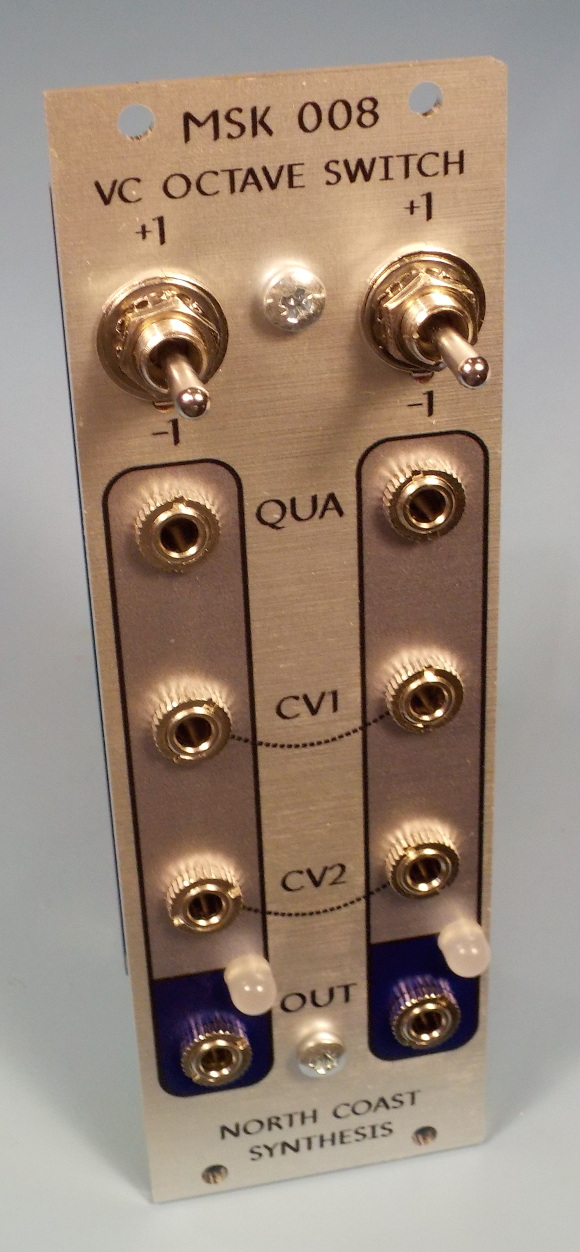
\includegraphics[width=\linewidth]{finished.jpg}
